\documentclass[12pt,titlepage]{article}
\usepackage[margin=1.25in]{geometry}
\usepackage{graphicx,amsmath}

%% Variables definition
\newcommand{\vSubject}{Matematika 3}
\newcommand{\vSubtitle}{Vectors}
\newcommand{\vName}{Dicha Zelianivan Arkana}
\newcommand{\vNIM}{2241720002}
\newcommand{\vClass}{2i}
\newcommand{\vDepartment}{Information Technology}
\newcommand{\vStudyProgram}{D4 Informatics Engineering}

%% [START] Tikz related stuff
\usepackage{tikz}
\usetikzlibrary{svg.path,calc,shapes.geometric,shapes.misc}
\tikzstyle{terminator} = [rectangle, draw, text centered, rounded corners = 1em, minimum height=2em]
\tikzstyle{preparation} = [chamfered rectangle, chamfered rectangle sep=0.75em, draw, text centered, minimum height = 2em]
\tikzstyle{process} = [rectangle, draw, text centered, minimum height=2em]
\tikzstyle{decision} = [diamond, aspect=2, draw, text centered, minimum height=2em]
\tikzstyle{data}=[trapezium, draw, text centered, trapezium left angle=60, trapezium right angle=120, minimum height=2em]
\tikzstyle{connector} = [line width=0.25mm,->]
%% [END] Tikz related stuff

%% [START] Fancy header related stuff
\usepackage{fancyhdr}
\pagestyle{fancy}
\setlength{\headheight}{15pt} % compensate fancyhdr style
\fancyhead{}
\fancyfoot{}
\fancyfoot[L]{\thepage}
\fancyfoot[R]{\textit{\vSubject - \vSubtitle}}
\renewcommand{\footrulewidth}{0.4pt}% default is 0pt, overline for footer
%% [END] Fancy header related stuff

%% [START] Custom tabular command related stuff
\usepackage{tabularx}
\newcommand{\details}[2]{
    #1 & #2  \\
}
%% [END] Custom tabular command related stuff

%% [START] Figure related stuff
\newcommand{\image}[3][1]{
    \begin{figure}[h]
        \centering
        \includegraphics[#1]{#2}
        \caption{#3}
        \label{#3}
    \end{figure}
}
%% [END] Figure related stuff

\begin{document}
\begin{titlepage}
    \centering
    \vfill
    {\bfseries\LARGE
        \vSubject\\
        \vskip0.25cm
        \vSubtitle
    }
    \vfill
    
\includegraphics[width=6cm]{images/polinema-logo.png}
    \vfill
    {
        \textbf{Name}\\
        \vName\\
        \vskip0.5cm
        \textbf{NIM}\\
        \vNIM\\
        \vskip0.5cm
        \textbf{Class}\\
        \vClass\\
        \vskip0.5cm
        \textbf{Department}\\
        \vDepartment\\
        \vskip0.5cm
        \textbf{Study Program}\\
        \vStudyProgram
    }
\end{titlepage}

\section{Questions}
\begin{enumerate}
    \item {
        If $z_1 = 5_i - 2_j, z_2 = 3_i + 3_j, z_3 = 4_i - 1_j$, determine:
        \begin{enumerate}
            \item {
                \begin{align*}
                    z_1 + z_2 + z_3 &= (5_i - 2_j) + (3_i + 3_j) + (4_i - 1_j) \\
                                    &= (5_i + 3_i + 4_i) + (-2_j + 3_j - 1_j) \\
                                    &= 12_i + 0_j \\
                                    &= 12_i
                \end{align*}
            }
            \item {
                \begin{align*}
                    z_1 - z_2 - z_3 &= (5_i - 2_j) - (3_i + 3_j) - (4_i - 1_j) \\
                                    &= (5_i - 3_i - 4_i) + (-2_j - 3_j + 1_j) \\
                                    &= -2_i - 4_j
                \end{align*}
            }
        \end{enumerate}
    }
    \item {
        If $\overline{OA} = 4_i + 3_j, \overline{OB} = 6_i - 2_j, \overline{OC} = 2_i - j$, determine
        $\overline{AB}, \overline{BC}, \overline{CA}$, and determine the lengths of the sides of triangle $ABC$.
        \begin{align*}
            \overline{AB} &= \overline{OB} - \overline{OA} \\
                            &= (6_i - 2_j) - (4_i + 3_j) \\
                            &= (6_i - 4_i) + (-2_j - 3_j) \\
                            &= 2_i - 5_j\\
            \overline{BC} &= \overline{OC} - \overline{OB} \\
                            &= (2_i - j) - (6_i - 2_j) \\
                            &= (2_i - 6_i) + (-j + 2_j) \\
                            &= -4_i + j\\
            \overline{CA} &= \overline{OA} - \overline{OC} \\
                            &= (4_i + 3_j) - (2_i - j) \\
                            &= (4_i - 2_i) + (3_j + j) \\
                            &= 2_i + 4_j
        \end{align*}
        The length of the triangle is calculated using the following formula:
        \begin{align*}
            \overline{AB} &= \sqrt{(2)^2 + (-5)^2} \\
                          &= \sqrt{4 + 25} \\
                          &= \sqrt{29} \\
                          &= 5.385 \\
            \overline{BC} &= \sqrt{(-4)^2 + (1)^2} \\
                          &= \sqrt{16 + 1} \\
                          &= \sqrt{17} \\
                          &= 4.123 \\
            \overline{CA} &= \sqrt{(2)^2 + (4)^2} \\
                          &= \sqrt{4 + 16} \\
                          &= \sqrt{20} \\
                          &= 4.472
        \end{align*}
    }
    \pagebreak
    \item {
        Determine the result of adding this vector along with its image:
        \begin{enumerate}
           \item {
                $\overline{PQ} + \overline{QR} + \overline{RS} + \overline{ST}$\\
                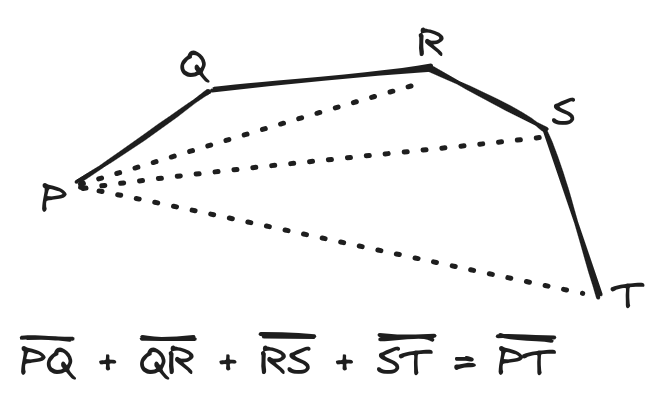
\includegraphics[height=4cm]{./images/vector-1.png}
           }
           \item {
                $\overline{AC} + \overline{CL} - \overline{ML}$\\
                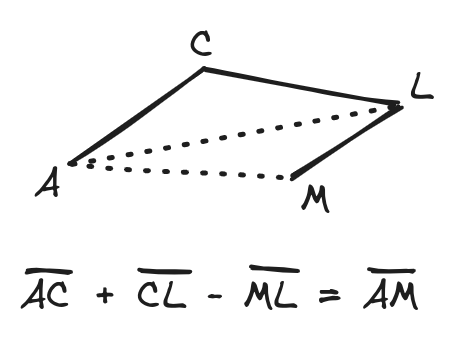
\includegraphics[height=4cm]{./images/vector-2.png}
           }
           \item {
                $\overline{GH} + \overline{HJ} + \overline{JK} + \overline{KL} + \overline{LG}$\\
                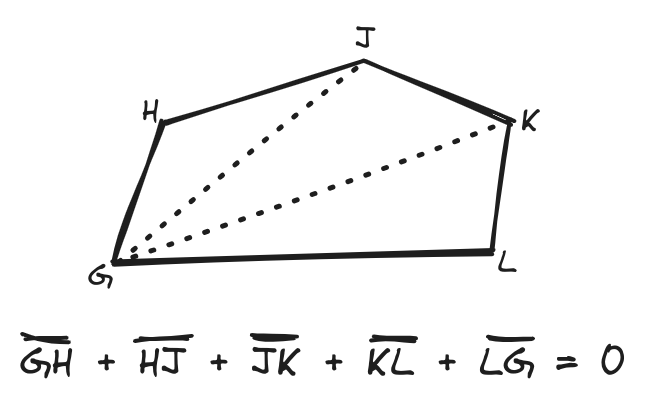
\includegraphics[height=4cm]{./images/vector-3.png}
           }
           \item {
                $\overline{AB} + \overline{BC} + \overline{CD} + \overline{DB}$\\
                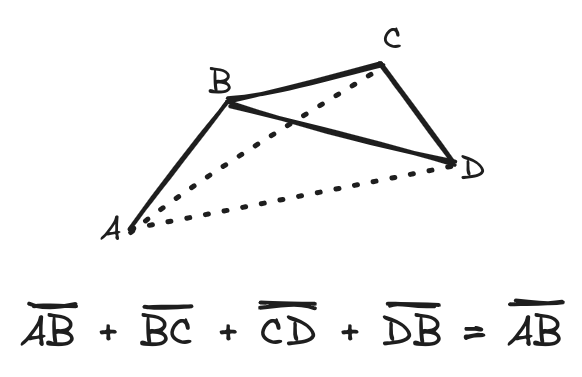
\includegraphics[height=4cm]{./images/vector-4.png}
           }
        \end{enumerate}
    }
\end{enumerate}

\end{document}

